

\tikzset{every picture/.style={line width=0.75pt}} %set default line width to 0.75pt        

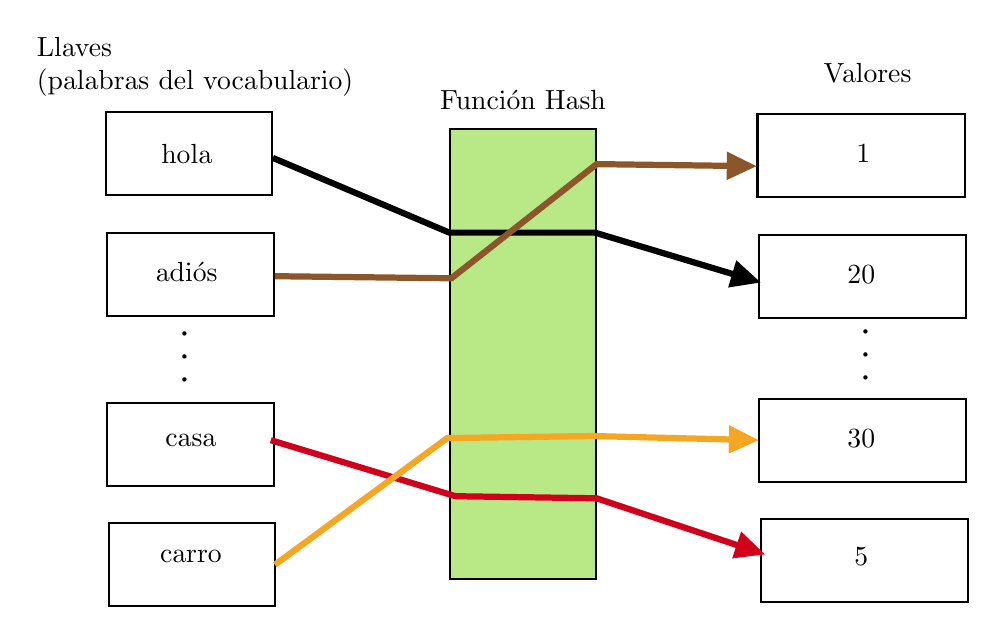
\begin{tikzpicture}[x=0.75pt,y=0.75pt,yscale=-1,xscale=1]
%uncomment if require: \path (0,334); %set diagram left start at 0, and has height of 334

%Shape: Rectangle [id:dp9405282177144714] 
\draw  [fill={rgb, 255:red, 184; green, 233; blue, 134 }  ,fill opacity=1 ] (253,50) -- (323,50) -- (323,267) -- (253,267) -- cycle ;
%Shape: Rectangle [id:dp8774923706333706] 
\draw   (401,43) -- (500.84,43) -- (500.84,83) -- (401,83) -- cycle ;
%Shape: Rectangle [id:dp09572839834830282] 
\draw   (401.83,101) -- (501.67,101) -- (501.67,141) -- (401.83,141) -- cycle ;
%Shape: Rectangle [id:dp1880999561103287] 
\draw   (401.83,180) -- (501.67,180) -- (501.67,220) -- (401.83,220) -- cycle ;
%Shape: Rectangle [id:dp4928306397366884] 
\draw   (402.66,238) -- (502.5,238) -- (502.5,278) -- (402.66,278) -- cycle ;
%Shape: Rectangle [id:dp06784076437826858] 
\draw   (87,42) -- (167.17,42) -- (167.17,82) -- (87,82) -- cycle ;
%Shape: Rectangle [id:dp9784309669414966] 
\draw   (87.67,100) -- (167.83,100) -- (167.83,140) -- (87.67,140) -- cycle ;
%Shape: Rectangle [id:dp34939452369495627] 
\draw   (87.67,182) -- (167.83,182) -- (167.83,222) -- (87.67,222) -- cycle ;
%Shape: Rectangle [id:dp41241321461007474] 
\draw   (88.33,240) -- (168.5,240) -- (168.5,280) -- (88.33,280) -- cycle ;
%Straight Lines [id:da9671353619044671] 
\draw [line width=2.25]    (167.5,64) -- (252.5,100) -- (322.68,100) -- (398.67,122.85) ;
\draw [shift={(402.5,124)}, rotate = 196.73] [fill={rgb, 255:red, 0; green, 0; blue, 0 }  ][line width=2.25]  [draw opacity=0] (14.29,-6.86) -- (0,0) -- (14.29,6.86) -- cycle    ;

%Straight Lines [id:da5193499988670736] 
\draw [color={rgb, 255:red, 139; green, 87; blue, 42 }  ,draw opacity=1 ][line width=2.25]    (168.5,121) -- (253.5,122) -- (323.5,67) -- (396.5,67.95) ;
\draw [shift={(400.5,68)}, rotate = 180.74] [fill={rgb, 255:red, 139; green, 87; blue, 42 }  ,fill opacity=1 ][line width=2.25]  [draw opacity=0] (14.29,-6.86) -- (0,0) -- (14.29,6.86) -- cycle    ;

%Straight Lines [id:da4044543016300448] 
\draw [color={rgb, 255:red, 208; green, 2; blue, 27 }  ,draw opacity=1 ][line width=2.25]    (166.5,200) -- (255.5,227) -- (323.5,228) -- (400.71,253.74) ;
\draw [shift={(404.5,255)}, rotate = 198.43] [fill={rgb, 255:red, 208; green, 2; blue, 27 }  ,fill opacity=1 ][line width=2.25]  [draw opacity=0] (14.29,-6.86) -- (0,0) -- (14.29,6.86) -- cycle    ;

%Straight Lines [id:da9966552915826332] 
\draw [color={rgb, 255:red, 245; green, 166; blue, 35 }  ,draw opacity=1 ][line width=2.25]    (168.5,260) -- (251.5,199) -- (321.5,198) -- (397.5,199.9) ;
\draw [shift={(401.5,200)}, rotate = 181.43] [fill={rgb, 255:red, 245; green, 166; blue, 35 }  ,fill opacity=1 ][line width=2.25]  [draw opacity=0] (14.29,-6.86) -- (0,0) -- (14.29,6.86) -- cycle    ;


% Text Node
\draw (288,36) node  [align=left] {Función Hash};
% Text Node
\draw (130,20) node  [align=left] {		Llaves \\(palabras del vocabulario)};
% Text Node
\draw (454,23) node  [align=left] {Valores};
% Text Node
\draw (126,62) node  [align=left] {hola};
% Text Node
\draw (126,119) node  [align=left] {adiós};
% Text Node
\draw (128,200) node  [align=left] {casa};
% Text Node
\draw (128,256) node  [align=left] {carro};
% Text Node
\draw (452,62) node  [align=left] {1};
% Text Node
\draw (451,120) node  [align=left] {20};
% Text Node
\draw (451,199) node  [align=left] {30};
% Text Node
\draw (451,256) node  [align=left] {5};
% Text Node
\draw (125,160) node [rotate=-90] [align=left] {\textbf{. . .}};
% Text Node
\draw (453,159) node [rotate=-90] [align=left] {\textbf{. . .}};


\end{tikzpicture}
